% !TeX root = ../main.tex
% Add the above to each chapter to make compiling the PDF easier in some editors.

\section{HMD Stencil Mask} \label{stencilmask}
Introduced to the mass market with 3Dlabs' Permedia II in 1997 and widely adopted since then, all modern graphics chips support a  useful feature called the stencil buffer. This buffer uses low bit integer values - commonly 8 bits per pixel for a depth of 256 \cite{deVries.2014} - which can be read from and written to during the fragment stage, with stencil testing happening after alpha and before depth testing. Sometimes used for certain shadowing operations, the stencil buffer is primarily used for cheap masking efforts. \\
One such effort was presented by Alex Vlachos at GDC 2015 \cite{Vlachos.2015} as a possibility to improve performance in \gls{VR} applications. Once again pointing at the significant areas of invisible screen space wasted outside the HMD lenses' warping reach (such as in \autoref{fig:stencil_wastecomparison}), the idea here is to write into a per-eye pixel matched stencil buffer a mask corresponding to the shape of the visible screen area. During the fragment stage of a frame render, the stencil test can early discard all masked fragments and thus avoid pixel shader work for all these areas. The operation works exactly as the classic idea of a stencil mask when painting surfaces. Paint will only hit the surface within the cutouts of the stencil. Similarly the graphics chip will only write color and depth values to unmasked fragments. 

\begin{figure}[h]
  \centering
  \hspace*{\fill}
     \subfloat[HTC Vive full render after warp\label{fig:stencil_allpixels}]{%
       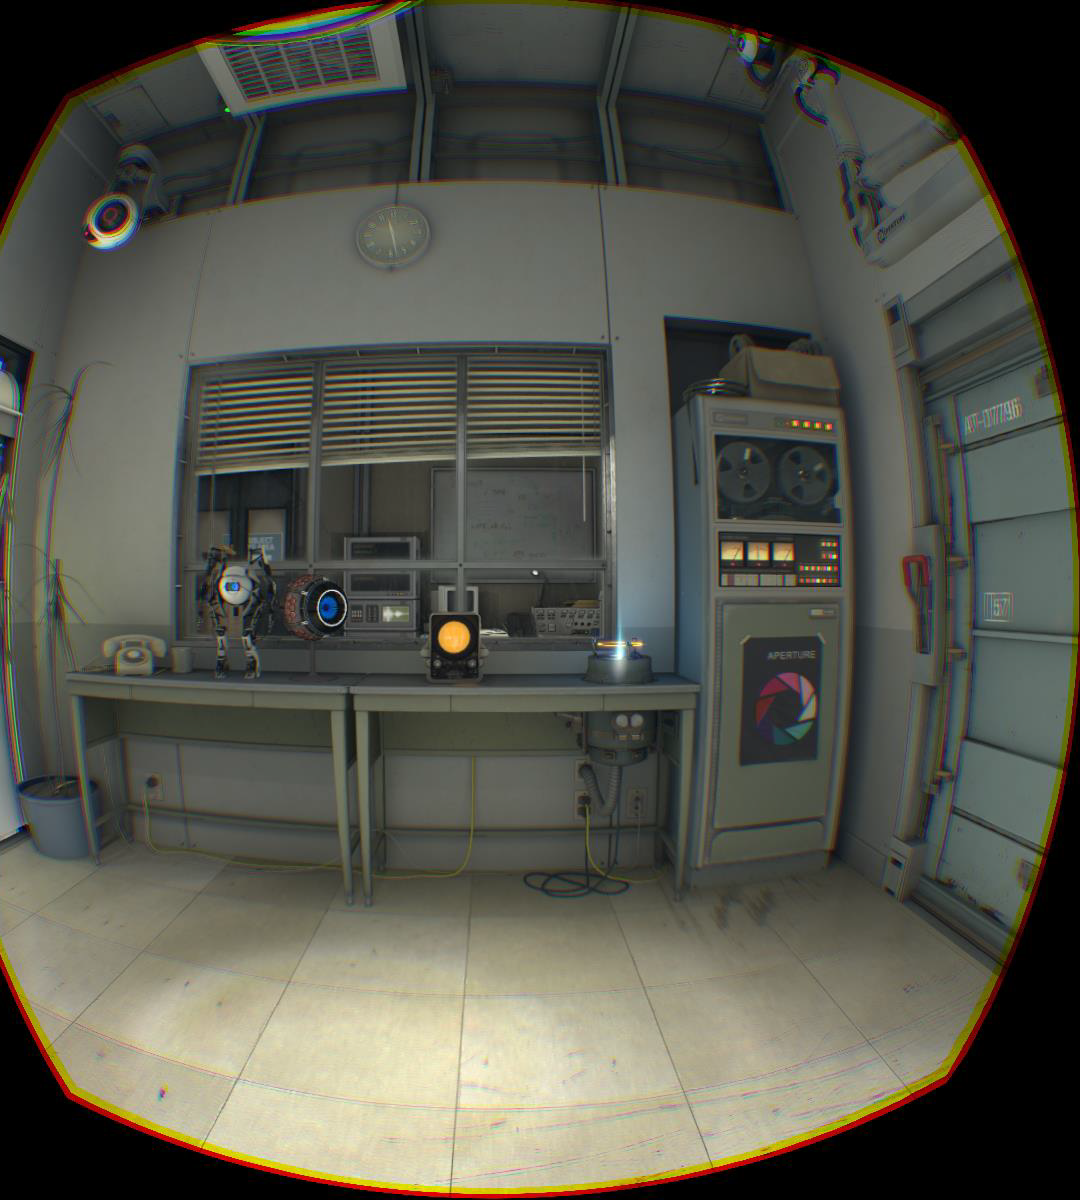
\includegraphics[width=0.4\textwidth]{pictures/vlachos_allpixels}
     }
  \hfill
     \subfloat[HTC Vive pixels wasted by lens cutout marked in red\label{fig:stencil_wastedpixels}]{%
       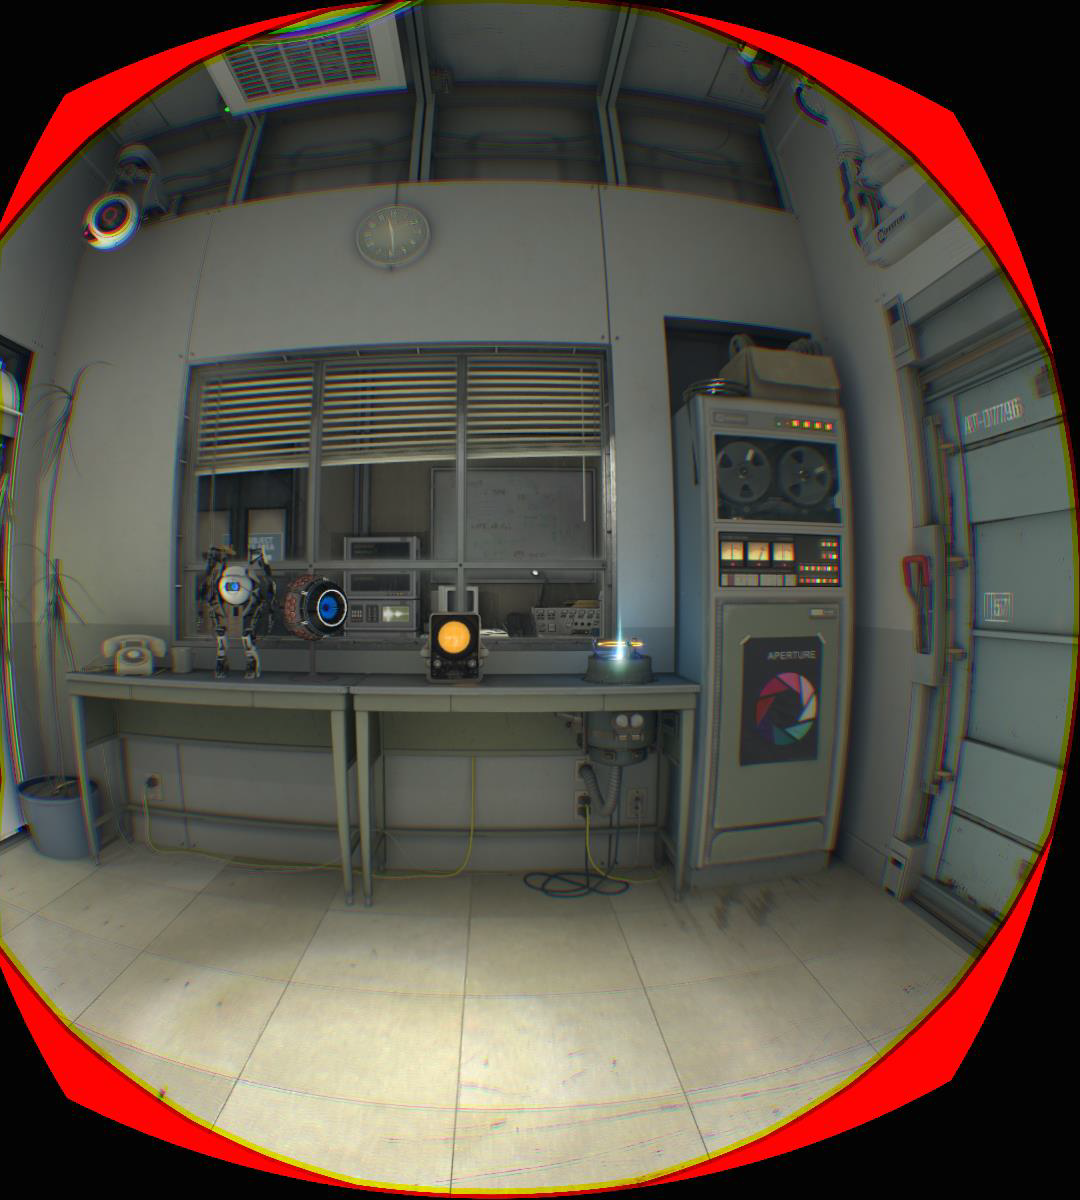
\includegraphics[width=0.4\textwidth]{pictures/vlachos_wastedpixels}
     }
  \hspace*{\fill}
     \caption{Comparison of rendered rectangular right eye frame after warp versus pixels wasted by lens distortion (from \cite{Vlachos.2015}, pp. 52-54, A. Vlachos. 2015)}
     \label{fig:stencil_wastecomparison}
\end{figure}

\begin{figure}[htb]
  \centering
  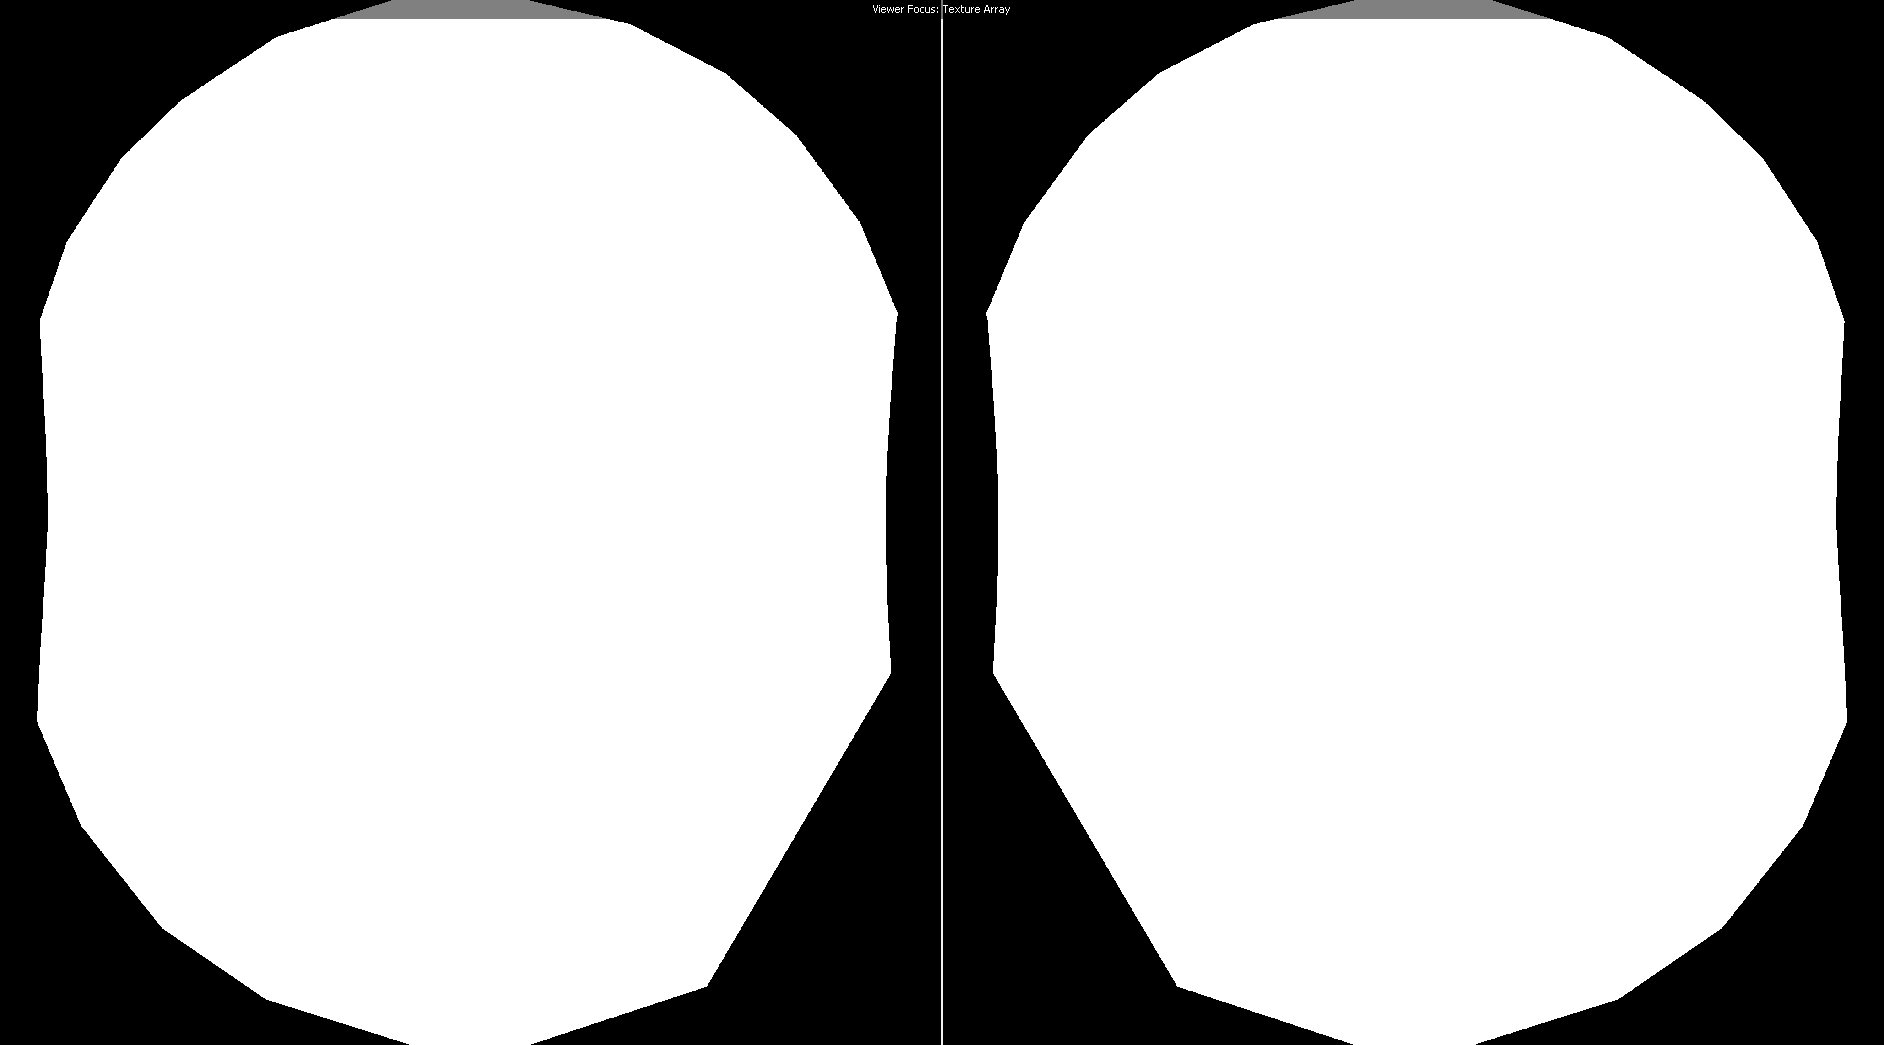
\includegraphics[width=0.9\textwidth]{pictures/stencilmask_Index_crop}
  \caption{\gls{Nsight VS} capture of stencil buffer as rendered for Valve Index \gls{HMD}} \label{fig:stencil_index}
\end{figure}

\subsection{Estimated impact}
The performance gain naturally scales well with both increased fragment shader bias of the per-frame workload as well as with the HMD's blind areas. In his GDC talk, Valve's Alex Vlachos, showcased gains of 17\% lower GPU fill rate for the company's Aperture Labs \gls{VR} showcase scene using an HTC Vive headset (\cite{Vlachos.2015}, p. 59). 
Assuming a roughly uniform distribution of objects in the scene and, accordingly, a roughly constant shader workload during use, the relative improvement in fragment render time is directly proportional to the masked percentage of the total framebuffer. 

\subsection{Implementation specifics}
The \gls{rtvklib} stencil masking feature is designed to query the require fitted meshes from OpenVR and render them to the respective eye at startup so the render loop can keep reusing it every frame without additional render load for the mask (see \autoref{fig:StencilMask}). An example of the rendered mask is shown in \autoref{fig:stencil_index}, displaying the \gls{Nsight VS} stencil buffer capture when using a Valve Index headset. \\
Outfitting \gls{Tachyon} for stencil masking required the addition of the entire stencil stack as the engine does not use the feature in any other capacity. The changes include extending the depth attachment of the OpenVR render pass with the \codeword{VK_IMAGE_ASPECT_STENCIL_BIT} so the additional buffer layer is created at startup. The involved Vulkan pipelines need stencil operation states defined in their \codeword{VkPipelineDepthStencilStateCreateInfo}, with the operations set as in \autoref{fig:lst_StencilOpState_MaterialPipeline} so the bits are checked against but not modified. Next, the \gls{VR} render pass needs its color attachment's \codeword{stencilLoadOp} set to \codeword{VK_ATTACHMENT_LOAD_OP_LOAD} so the renderer knows to load the stencil buffer at the start of the color pass, and the \codeword{stencilStoreOp} to \codeword{VK_ATTACHMENT_STORE_OP_DONT_CARE} so it can leave the buffer behind after use without saving anything more to it. This is important to make sure the stencil buffer remains unmodified and expensive writes are avoided. 

\begin{figure}[htb]
  \centering
  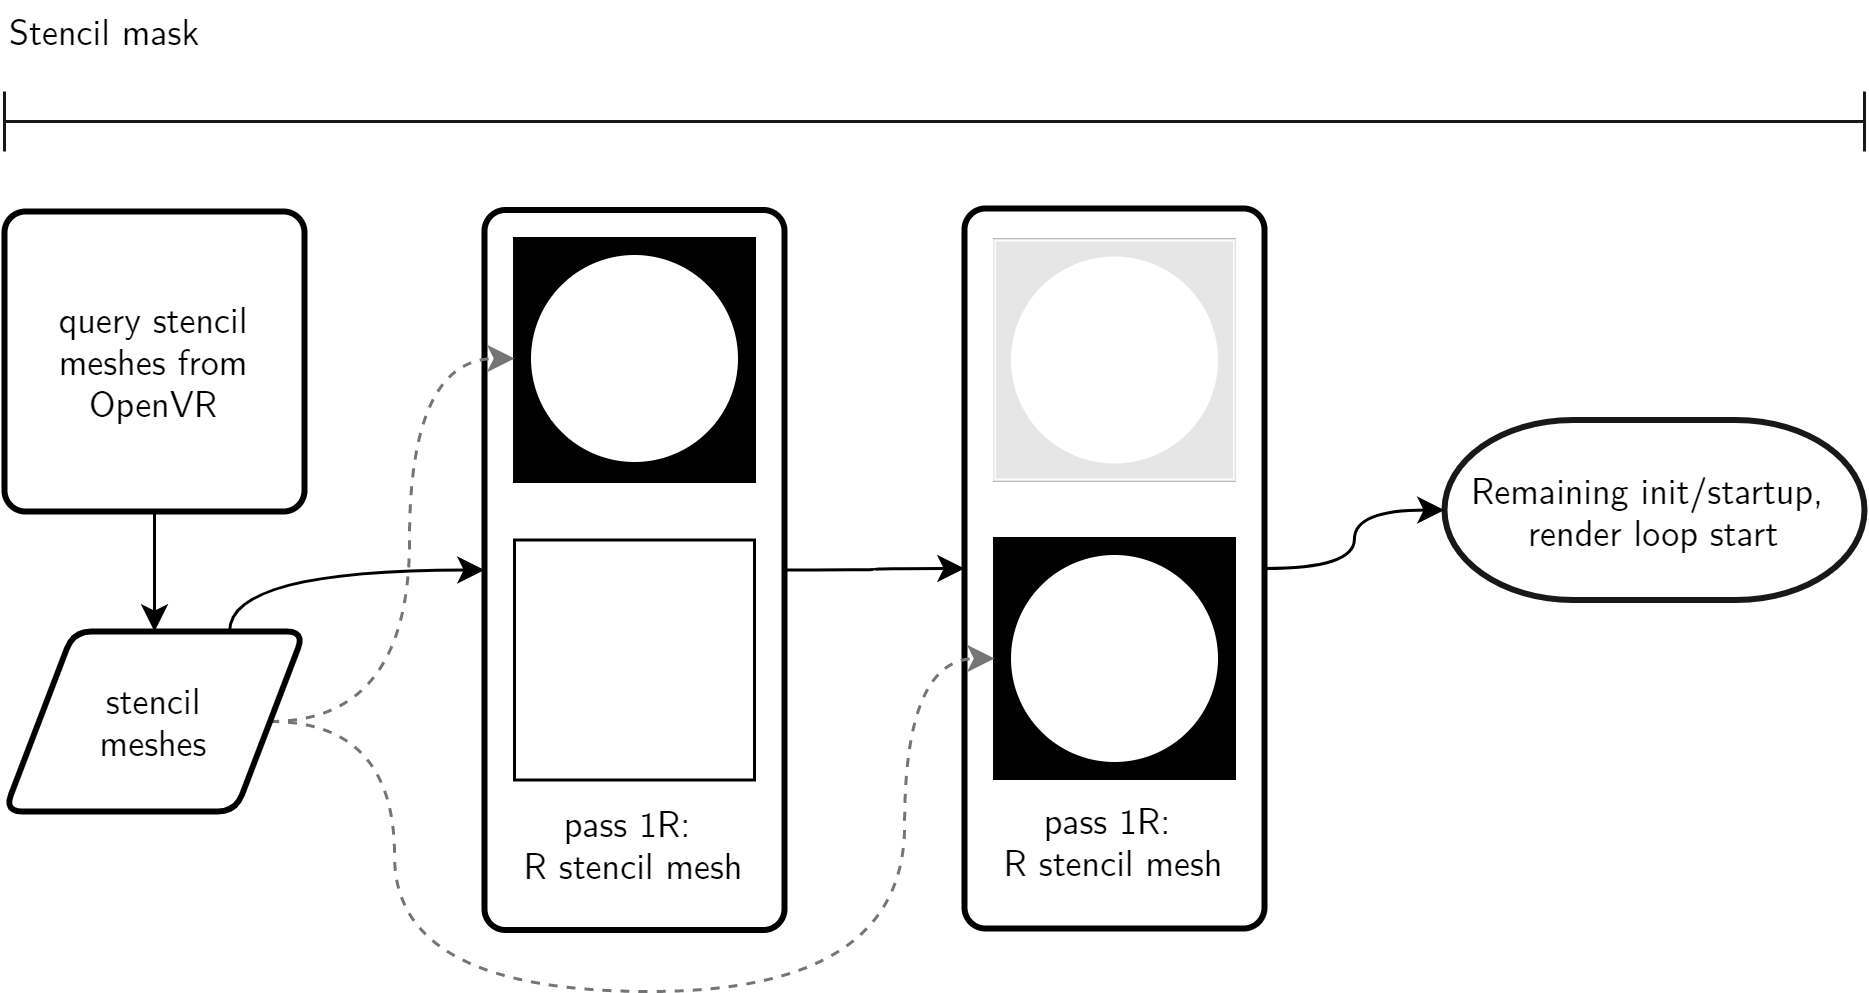
\includegraphics[width=0.9\textwidth]{pictures/StencilMask}
  \caption{HMD stencil mask query and render flow in \gls{rtvklib}} \label{fig:StencilMask}
\end{figure}

\begin{figure}[htb]
  \centering
  \begin{tabular}{c}
  \begin{lstlisting}[language=C++]
	//stencil op settings for pipelines using 
	//the stencil mask for comparison 
	VkStencilOpState stencilOpState = {};
	stencilOpState.compareOp = VK_COMPARE_OP_NOT_EQUAL;
	stencilOpState.failOp = VK_STENCIL_OP_KEEP;
	stencilOpState.depthFailOp = VK_STENCIL_OP_KEEP;
	stencilOpState.passOp = VK_STENCIL_OP_KEEP;
	stencilOpState.compareMask = 0xff;
	stencilOpState.writeMask = 0xff;
	stencilOpState.reference = 1;
	\end{lstlisting}
  \end{tabular}
  \caption[Material pipeline stencil operation flags]{Stencil operation flags set for default material Pipeline}\label{fig:lst_StencilOpState_MaterialPipeline}
\end{figure}

Rendering the stencil mask itself at startup is done as follows: 
OpenVR by now has some helper functions for masking built in, such as the \codeword{GetHiddenAreaMesh(EVREye eEye)} function that returns a screenspace-normalized list of vertices representing the ideal mask mesh for the current HMD if available to OpenVR. Exceptions apply, as the API does not contain mask definitions for all headsets. As an example, the mesh query returns an empty list for the Oculus Rift CV1 as seen in \autoref{fig:empty_mask}. With this in mind, the main benefit is the simplicity of getting a fitted mask for most HMDs instead of either approximating with circular masks or going through the trouble of manually creating fitted meshes for existing and upcoming OpenVR-enabled headsets. For exception cases a fast circular approximation mask may be an adequate compromise. \\
\gls{Tachyon} queries OpenVR for the mesh of each eye, converts the vertex lists into a renderer-compatible vertex format and writes out a vertex and index buffer each. 
At the end of the \gls{VR} render pass, an ad-hoc command buffer is recorded and submitted to render the two masks into the \gls{VR} framebuffer's depth attachment's stencil layer. The \codeword{VK_IMAGE_ASPECT_STENCIL_BIT} is set to ensure only that layer is written to. 

\begin{figure}[h]
  \centering
  \hspace*{\fill}
     \subfloat[Stencil mask returned for Valve Index]{%
       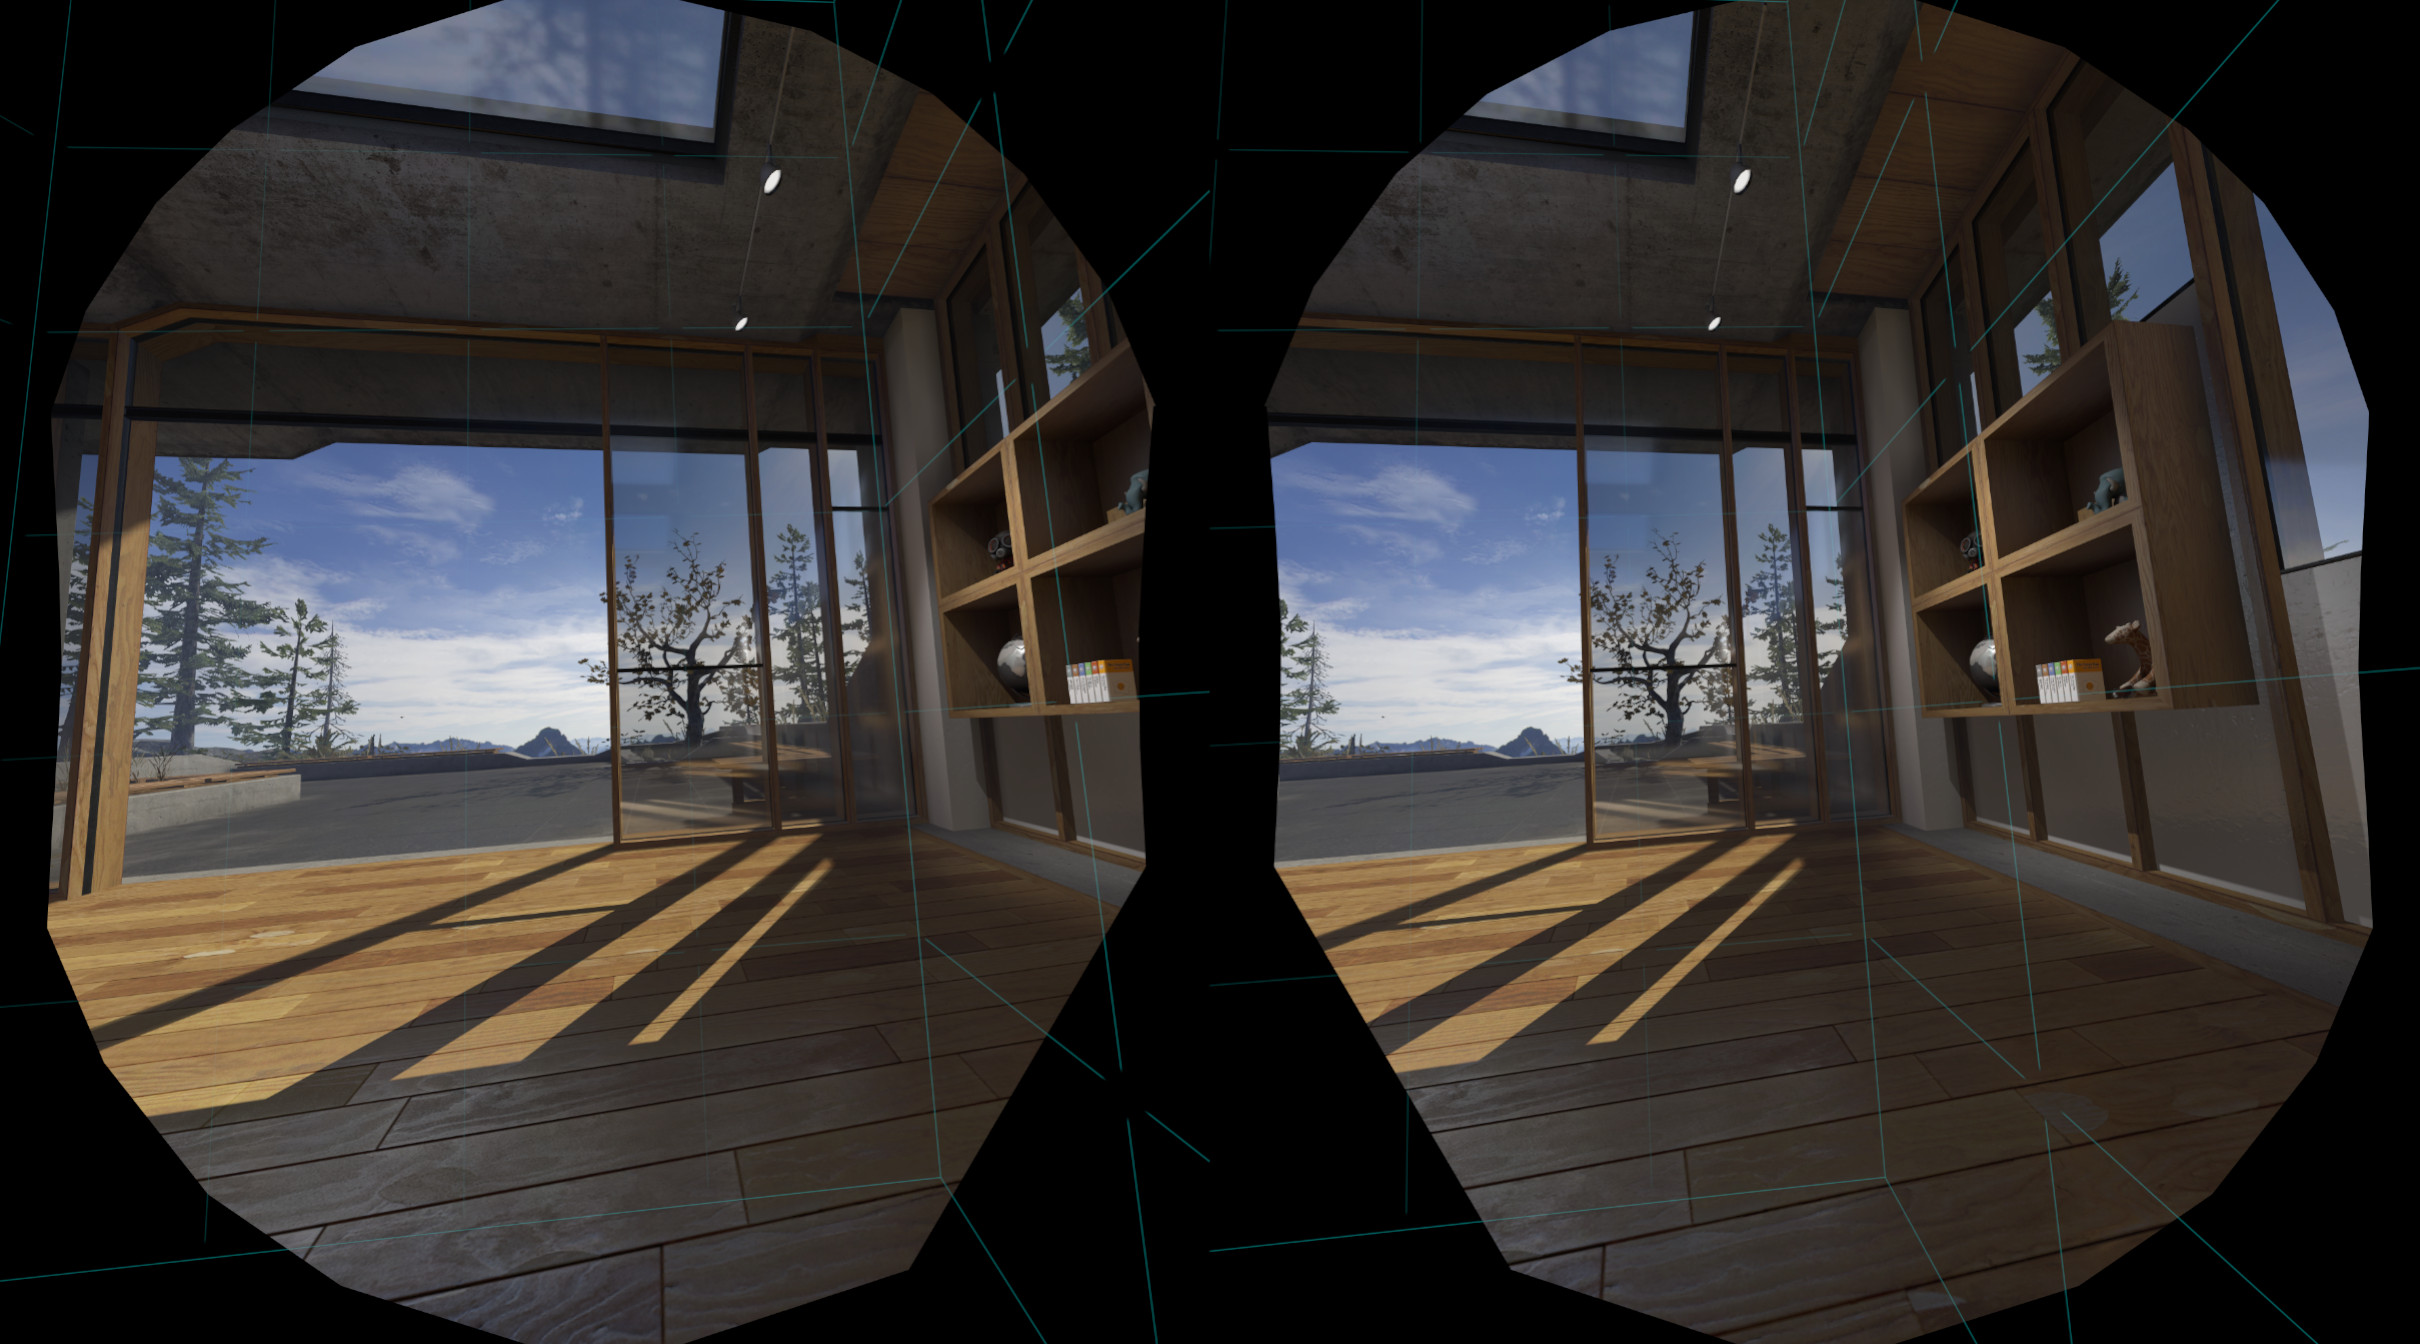
\includegraphics[width=0.4\textwidth]{pictures/index_home}
     }
  \hfill
  	\subfloat[Stencil mask returned for Samsung Odyssey]{%
       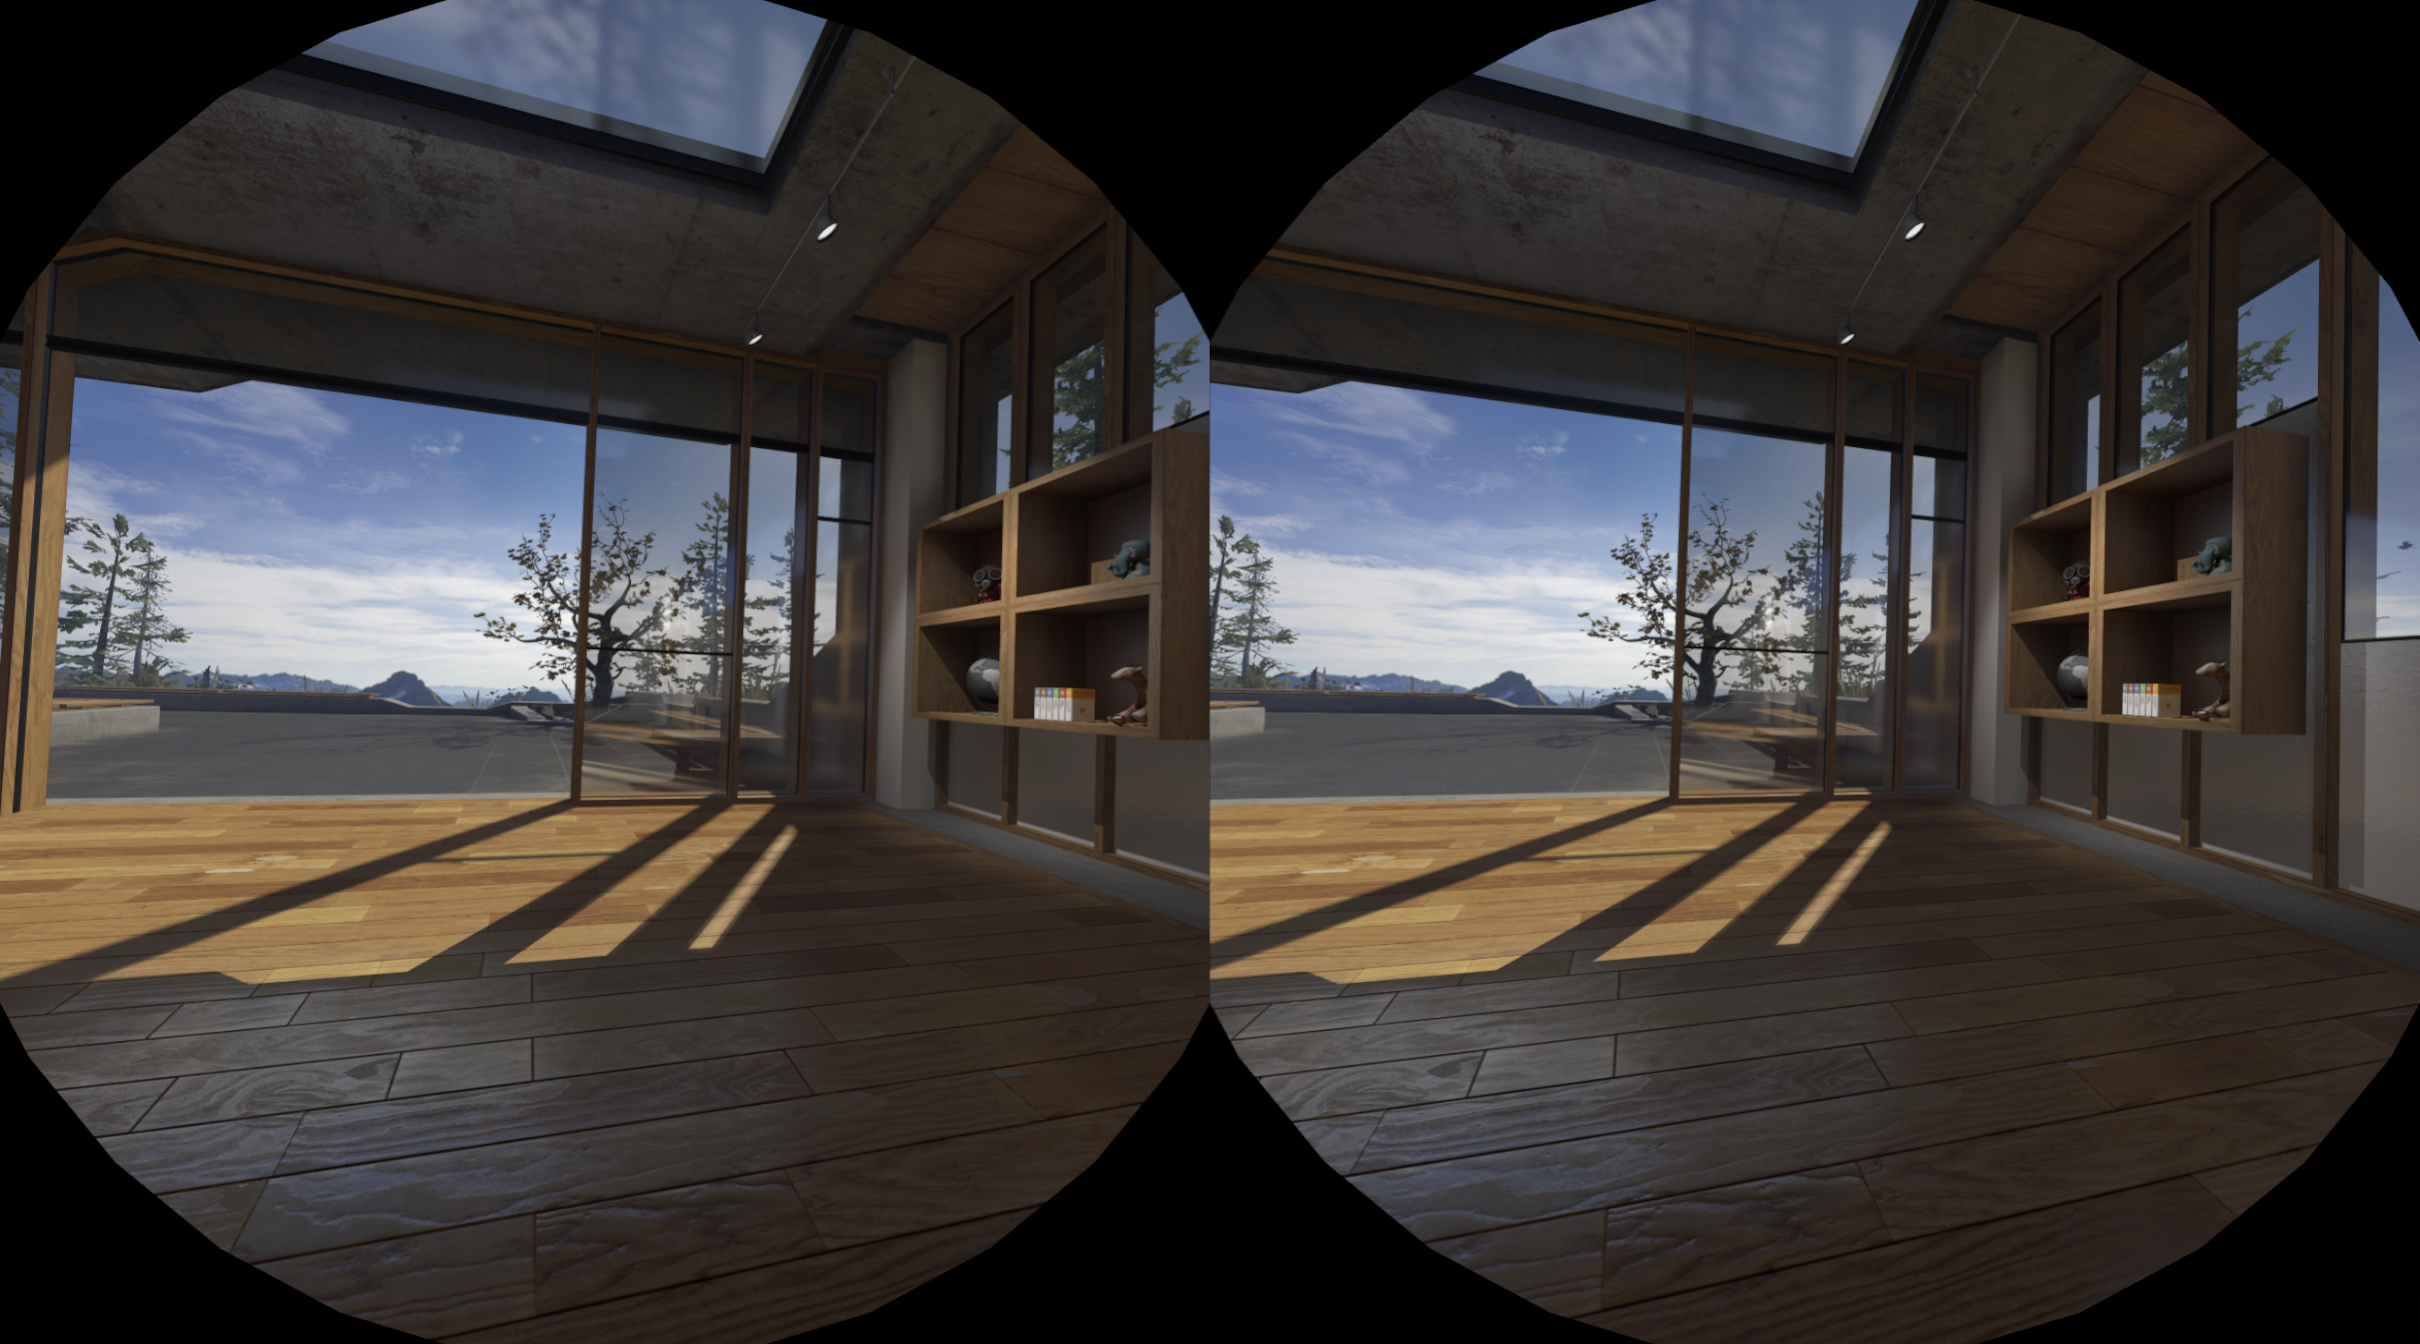
\includegraphics[width=0.4\textwidth]{pictures/odyssey_home}
     }
  \hspace*{\fill}
     \\
  \hspace*{\fill}
     \subfloat[Stencil mask returned for HTC Vive\textcolor{red}{[TODO: img]}]{%
       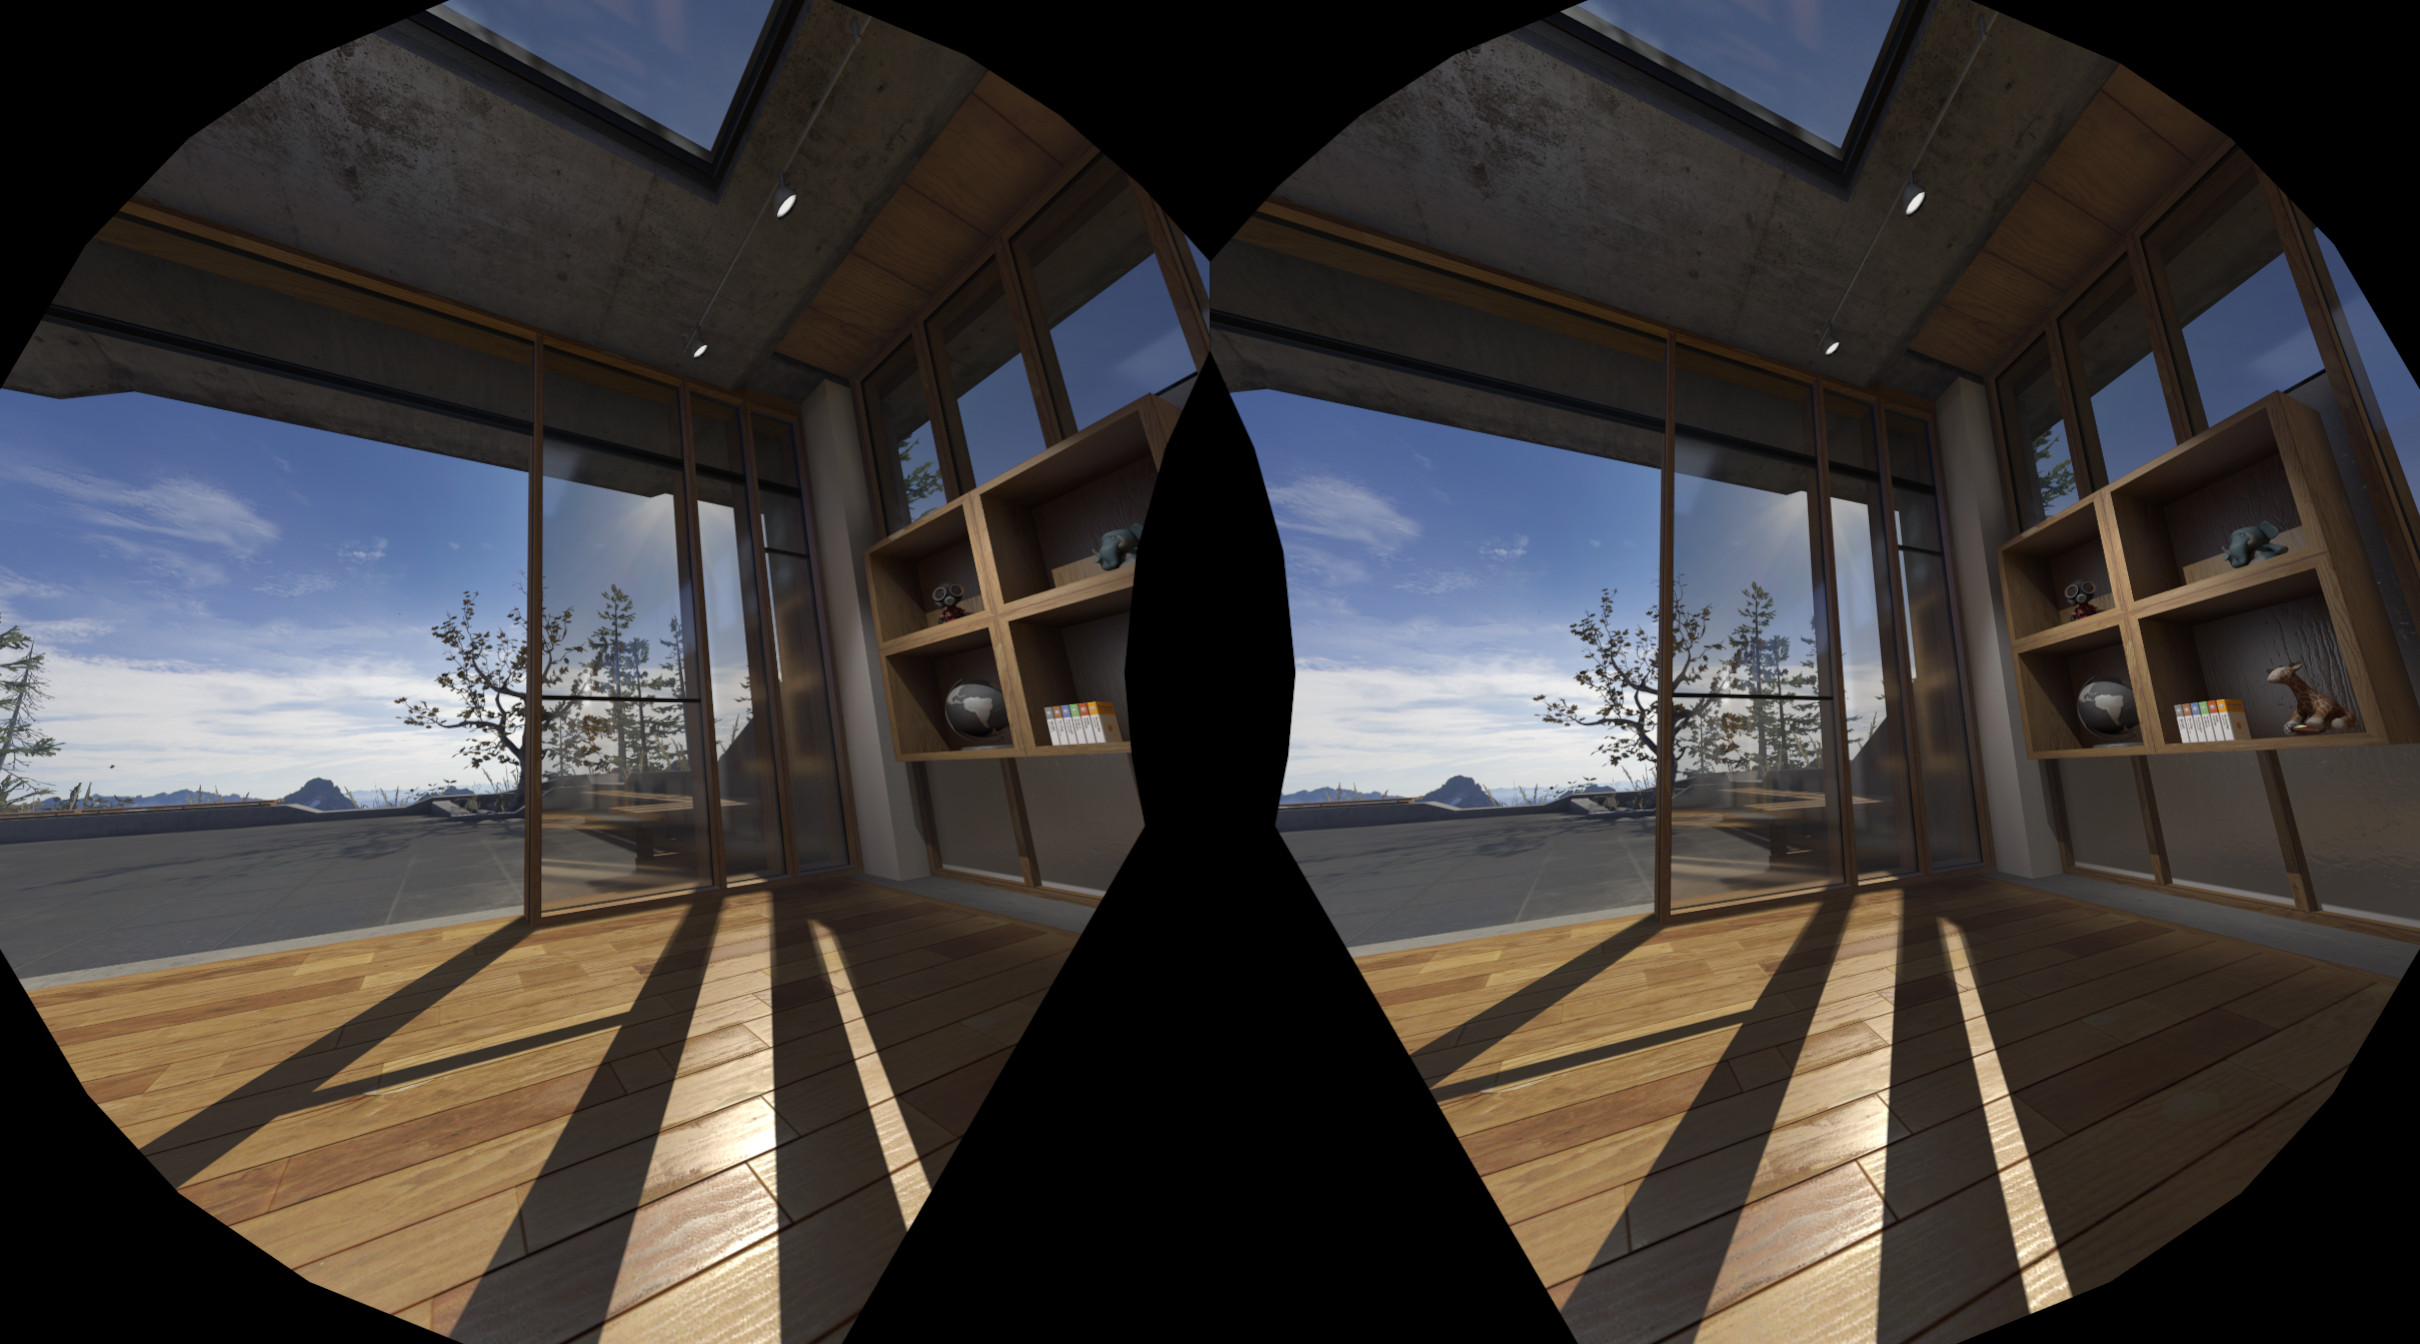
\includegraphics[width=0.4\textwidth]{pictures/vive_home}
     }
  \hfill
  	\subfloat[(lack of) Stencil mask returned for Oculus Rift CV1]{%
       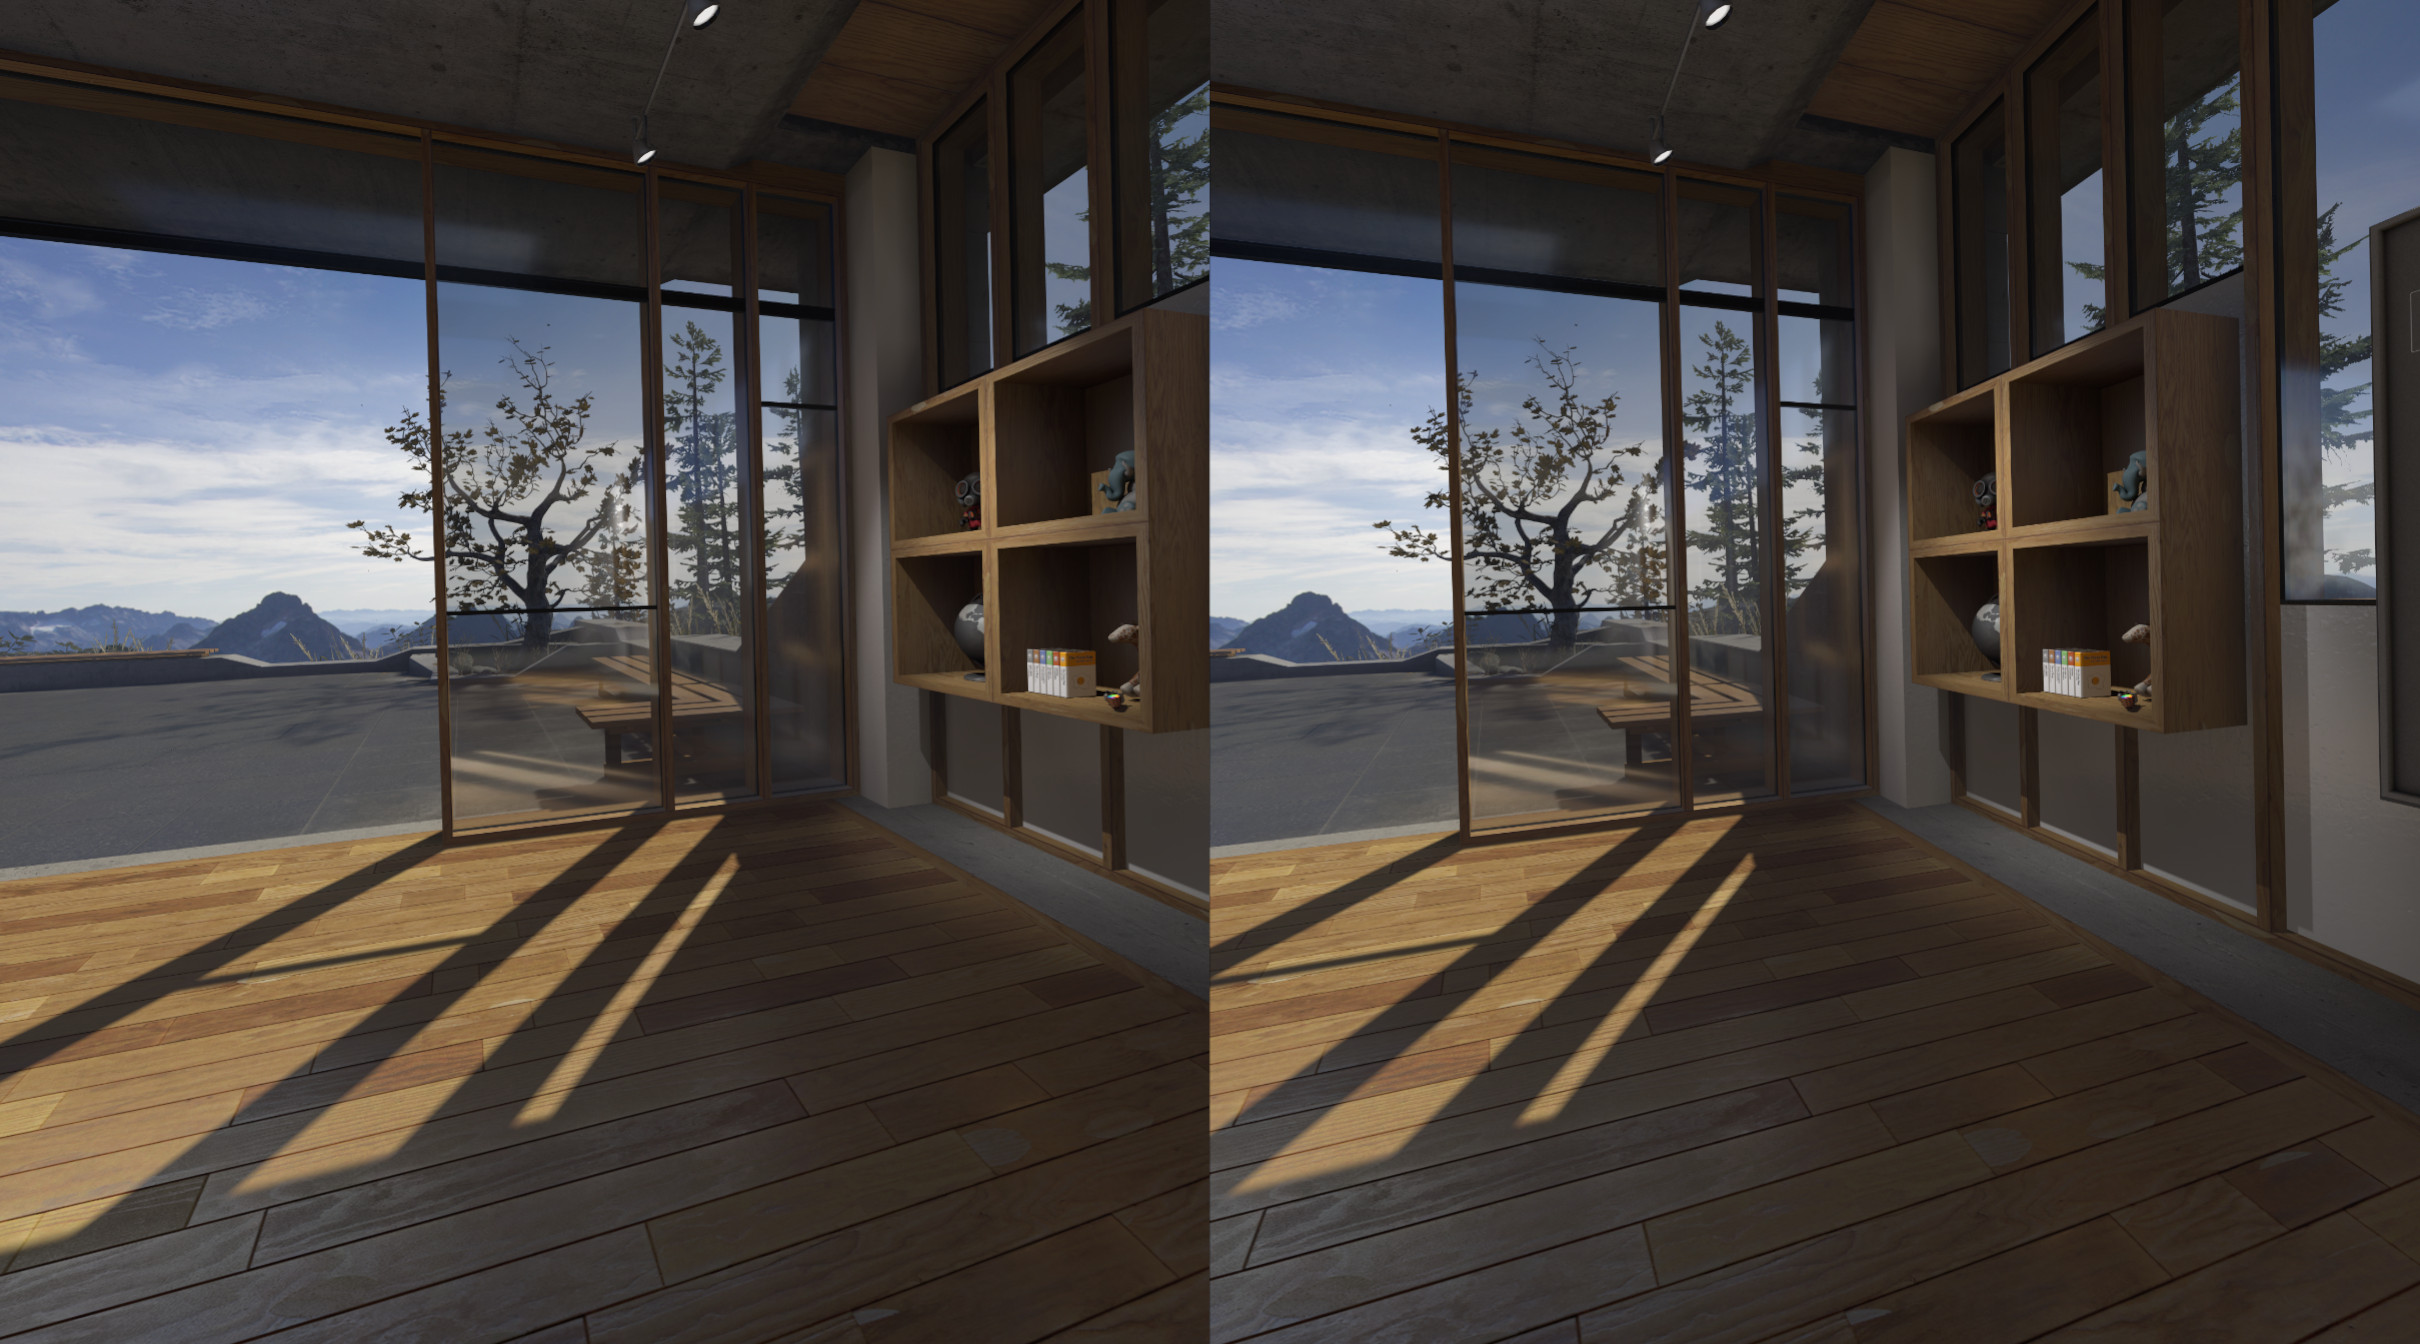
\includegraphics[width=0.4\textwidth]{pictures/rift_home}
     }
  \hspace*{\fill}
     \caption{Comparison of stencil mask availability (while running SteamVR home)}
     \label{fig:empty_mask}
\end{figure}

Due to Vulkan's verbose nature, rendering these two masks also requires its own pipeline. The default material and PBR pipelines only do stencil test compares, no writes and they perform color writes and rasterizer face culling, which are all things the stencil mask pipeline should do differently. A separate stencil pipeline is introduced with the stencil operation state set like in \autoref{fig:lst_StencilOpState_StencilPipeline}, the color writes masked off and rasterizer culling disabled. Should the need to perform per-frame stencil writes arise, merging the material pipelines and the stencil pipeline may prove beneficial to avoid expensive pipeline re-binds but for the sake of cleaner separation the described setup was used in \gls{Tachyon}'s current implementation. 

\begin{figure}[htb]
  \centering
  \begin{tabular}{c}
  \begin{lstlisting}[language=C++]
	//stencil op settings for the stencil pipeline 
	VkStencilOpState stencilOpState = {};
	stencilOpState.compareOp = VK_COMPARE_OP_ALWAYS;
	stencilOpState.failOp = VK_STENCIL_OP_REPLACE;
	stencilOpState.depthFailOp = VK_STENCIL_OP_REPLACE;
	stencilOpState.passOp = VK_STENCIL_OP_REPLACE;
	stencilOpState.compareMask = 0xff; 
	stencilOpState.writeMask = 0xff;
	stencilOpState.reference = 1;
	\end{lstlisting}
  \end{tabular}
  \caption[Stencil pipeline stencil operation flags]{Stencil operation flags set for stencil mask Pipeline}\label{fig:lst_StencilOpState_StencilPipeline}
\end{figure}
